\documentclass[a4paper,12pt]{article}
\usepackage[top = 2.5cm, bottom = 2.5cm, left = 2.5cm, right = 2.5cm]{geometry}
% Unfortunately, LaTeX has a hard time interpreting German Umlaute. The following two lines and packages should help. If it doesn't work for you please let me know.
\usepackage[T1]{fontenc}
\usepackage[utf8]{inputenc}
% The following two packages - multirow and booktabs - are needed to create nice looking tables.
\usepackage{multirow} % Multirow is for tables with multiple rows within one cell.
\usepackage{booktabs} % For even nicer tables.
% As we usually want to include some plots (.pdf files) we need a package for that.
\usepackage{graphicx}
% The default setting of LaTeX is to indent new paragraphs. This is useful for articles. But not really nice for homework problem sets. The following command sets the indent to 0.
\usepackage[spanish]{babel}
\usepackage{setspace}
\setlength{\parindent}{0in}
% Package to place figures where you want them.
\usepackage{float}
% The fancyhdr package let's us create nice headers.
\usepackage{fancyhdr}
\usepackage{amsmath}
\usepackage{amssymb}
\usepackage{natbib}
\usepackage{graphicx}
\usepackage{subcaption}
\usepackage{booktabs}
\usepackage{etoolbox}
\usepackage{amsthm}
\newenvironment{solution}
  {\renewcommand\qedsymbol{$\blacksquare$}\begin{proof}[Solución]}
  {\end{proof}}
\pagestyle{fancy}

\fancyhf{}

\lhead{\footnotesize Hoja de trabajo 1}
\rhead{\footnotesize  Rompich}
\cfoot{\footnotesize \thepage}



\begin{document}
    \thispagestyle{empty} % This command disables the header on the first page.

    \begin{tabular}{p{15.5cm}} % This is a simple tabular environment to align your text nicely
    \begin{tabbing}
    Universidad del Valle de Guatemala \\ 10 de febrero de 2021  \\
    Rudik R. Rompich   - Carné: 19857\\
    \end{tabbing}
    Estadística 2 - Eugenio Aristondo \\
    \hline % \hline produces horizontal lines.
    \\
    \end{tabular} % Our tabular environment ends here.
    \vspace*{0.3cm} % Now we want to add some vertical space in between the line and our title.
    \begin{center} % Everything within the center environment is centered.
    {\Large \bf Tarea 1 
} % <---- Don't forget to put in the right number
        \vspace{2mm}
    \end{center}
    \vspace{0.4cm}

\section{Sección 14}
\subsection{Ejercicio 9}
\begin{itemize}
    \item Trace un diagrama de dispersión utilizando el precio como la variable independiente.
    \begin{center}
        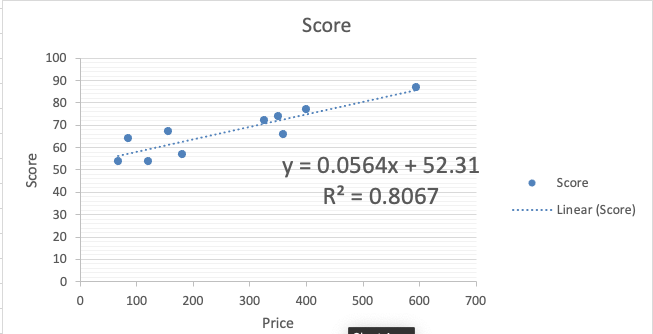
\includegraphics[scale=0.5]{Imagenes/9-1.png}
    \end{center}
    \item ¿Qué indica el diagrama de dispersión del inciso a) acerca de la relación entre las dos variables?
    \begin{solution}
    Indica que tiene una relación positiva.
    \end{solution}
    
    \item Use el método de mínimos cuadrados para desarrollar la ecuación de regresión estimada.
    \begin{center}
        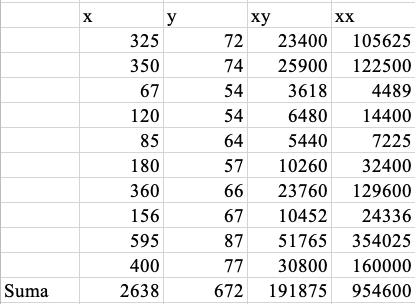
\includegraphics[scale=0.5]{Imagenes/9-2.png}
    \end{center}
    \begin{align}
\begin{array}{l}
intercepto=\frac{\sum Y \cdot \sum X^{2}-\sum X \cdot \sum X Y}{n \cdot \sum X^{2}-\left(\sum X\right)^{2}}=\frac{672 \cdot 954600-2638 \cdot 191875}{10 \cdot 954600-2638^{2}} \approx 52.31 \\
pendiente=\frac{n \cdot \sum X Y-\sum X \cdot \sum Y}{n \cdot \sum X^{2}-\left(\sum X\right)^{2}}=\frac{10 \cdot 191875-2638 \cdot 672}{10 \cdot 954600-(2638)^{2}} \approx 0.056
\end{array}
\end{align}

   $$\implies y= mx+b$$
   $$\implies y= 0.056x+52.31$$
    \item Proporcione una interpretación para la pendiente de la ecuación de regresión estimada.
    \begin{solution}
    Indica que por cada dolar hay un incremento de 0.056.
    \end{solution}
    \item  La maleta de la marca Eagle Creek Hovercraft tiene un precio de \$225. Usando la ecuación de regresión estimada desarrollada en el inciso c), prediga la puntuación para esta maleta.
    \begin{solution}
    $$\implies y= 0.056x+52.31$$
    $$\implies y= 0.056(225)+52.31$$
    $$\implies y= 64.91$$
    \end{solution}
\end{itemize}
\subsection{Ejercicio 19}
\begin{itemize}
    \item Calculelas SCE, STC y SCR.
    \begin{center}
        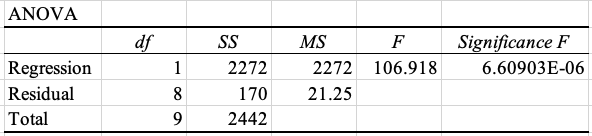
\includegraphics[scale=0.5]{Imagenes/19-1.png}
    \end{center}
    \begin{solution}
    \begin{itemize}
        \item SCE = 170
        \item SCR = 2272
        \item STC = 2442
    \end{itemize}
    \end{solution}
     \item Calcule el coeficiente de determinación $r^2$ . Haga un comentario sobre la bondad del ajuste.
     \begin{solution}
     Dado: 
     $$r^2= \frac{SCR}{STC}*100= \frac{2272}{2442}*100=93.04\% $$
     Eso quiere decir que el modelo explica el 93.04 de la variabilidad de $x$ y $y$. 
     \end{solution}
     \item ¿Cuál es el valor del coeficiente de correlación muestral?
     \begin{solution}
     $$r=\sqrt{0.9304}=0.9646$$
     \end{solution}
\end{itemize}
\subsection{Ejercicio 27}
\begin{itemize}
    \item  Use estos datos para desarrollar la ecuación de regresión estimada a efecto de estimar el precio de las mochilas y las botas para excursionismo con base en el soporte superior.
    \begin{center}
        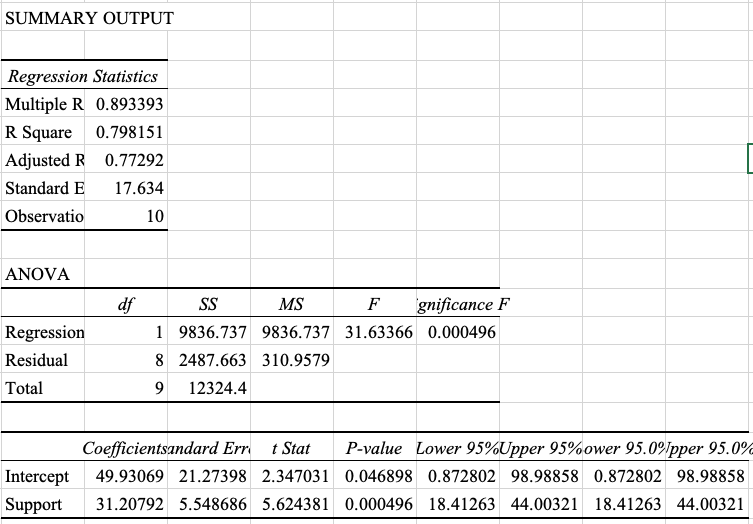
\includegraphics[scale=0.5]{Imagenes/27-1.png}
    \end{center}
    $$y=31,20792x+49,93069$$
    \item  Empleando un nivel de significancia de 0.05, determine si hay relación entre soporte superior y precio.
    \begin{solution}
    Basándose en el Valor-P, la $H_0$ se rechaza ya que el Valor-P $\leq 0.05$. 
    \end{solution}


    \item ¿Confiaría en usar la ecuación de regresión estimada desarrollada en el inciso a) para estimar el precio de las mochilas y las botas con base en la evaluación del soporte superior?
    \begin{solution}
    No, ya que el Valor-P de la pendiente no es significante.
    \end{solution}
    \item  Estime el precio de una mochila que tiene 4 como evaluación del soporte superior.
    
    \begin{solution}
    $$y=31,20792x+49,93069$$
    $$y=31,20792(4)+49,93069$$
    $$y= 165,4$$
    \end{solution}
\end{itemize}

\subsection{Ejercicio 44}
\begin{itemize}
    \item  Trace un diagrama de dispersión usando el peso como variable independiente.
    \begin{center}
        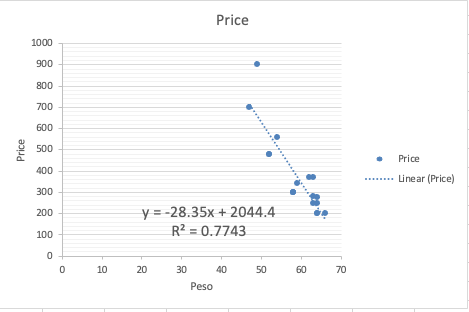
\includegraphics[scale=0.5]{Imagenes/44-1.png}
    \end{center}
    \item ¿Parece haber alguna relación entre las dos variables?
    \begin{solution}
    Sí, una relación negativa.
    \end{solution}
    \item c) Obtenga la ecuación de regresión estimada que pueda utilizarse para predecir el precio de acuerdo con el peso.
    \begin{center}
         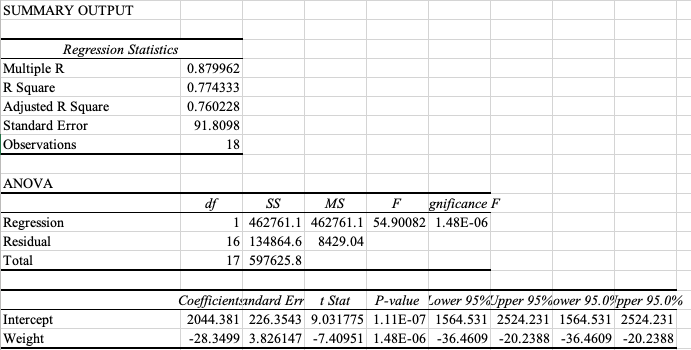
\includegraphics[scale=0.5]{Imagenes/44-3.png}
    \end{center}
    $$y=-28,3499x+2044,381$$
    \item Pruebe la significancia de la relación en un nivel de significancia de 0.05.
    \begin{solution}
    Basándose en el Valor-P, la $H_0$ se rechaza ya que el Valor-P $\leq 0.05$. 
    \end{solution}

    \item  ¿La ecuación de regresión estimada proporciona un buen ajuste? Explique.
    \begin{solution}
    $$r^2= \frac{SCR}{STC}*100= \frac{462761}{134864}*100=77,43\% $$
    Por lo que la regresión proporciona un buen ajuste.
    \end{solution}
\end{itemize}
\subsection{Ejercicio 49}
\begin{itemize}
    \item Obtenga una ecuación de regresión estimada que pueda utilizarse para pronosticar los precios de venta dada la extensión en pies cuadrados.
    \begin{center}
        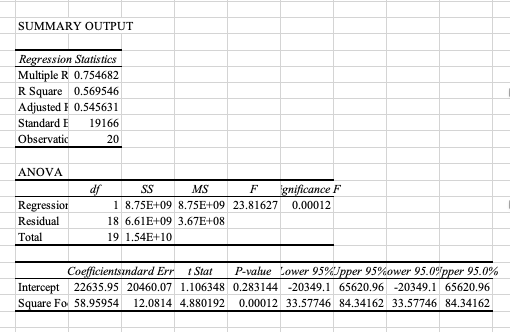
\includegraphics[scale=0.7]{Imagenes/49-1.png}
    \end{center}
    $$y=58,95954x+22635,95$$
    \item Construya una gráfica de residuales estandarizados contra la variable independiente.
    \begin{center}
        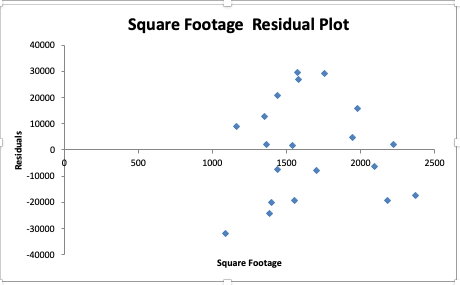
\includegraphics[scale=0.7]{Imagenes/49-2.png}
    \end{center}
    \item A la luz de la gráfica, ¿los supuestos acerca de los términos del error y de la forma del modelo parecen razonables?
    \begin{solution}
    No, pareciera que la gráfica no tiene una forma definida.
    \end{solution}
\end{itemize}

\section{Sección 15}

\subsection{Ejercicio 10}
\begin{itemize}
    \item  Desarrolle una ecuación de regresión estimada para predecir la proporción de juegos ganados, dada la proporción de anotaciones de campo del equipo.
    \begin{center}
        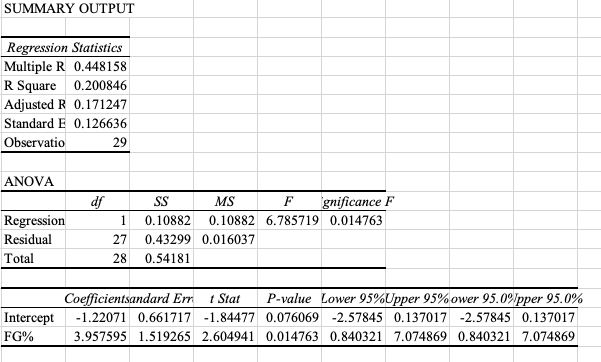
\includegraphics[scale=0.5]{Imagenes/50-10.png}
    \end{center}
    $$y=3,957595x-1,22071$$
    \item Interprete la pendiente de la ecuación de regresión estimada obtenida con el inciso a).
    \begin{solution}
    Quiere decir que por cada proporción de anotaciones de campo del equipo, hay un incremento de 3,957595 en la proporción de juegos ganados.
    \end{solution}
    \item Obtenga una ecuación de regresión estimada para predecir la proporción de juegos ganados dada la proporción de anotaciones de campo del equipo, el porcentaje de tiros de tres puntos del equipo contrario y el número de pérdidas de balón del equipo adversario.
    \begin{center}
        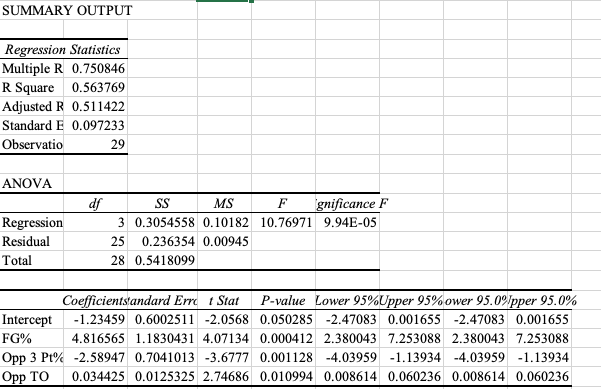
\includegraphics[scale=0.5]{Imagenes/50-10-1.png}
    \end{center}
    $$y=4,816565x_1-2,58947x_2+0,034425x_3-1,23459$$
    
    \item Analice las implicaciones prácticas de la ecuación obtenida en el inciso c).
    \begin{solution}
    Es un modelo con un $R^2$ bastante malo. No predice perfectamente la relación lineal.
    \end{solution}
    \item Estime la proporción de juegos ganados por un equipo para el que los valores de las tres variables independientes son: FG\% = 0.45; Opp 3 Pt\%= 0.34, y Opp TO =17.
    $$y=4,816565x_1-2,58947x_2+0,034425x_3-1,23459$$
    $$y=4,816565(0,45)-2,58947(0,34)+0,034425(17)-1,23459$$
    $$y=0,638$$
\end{itemize}
\subsection{Ejercicio 18}
\begin{itemize}
    \item a) En el inciso c) del ejercicio 10 se obtuvo una ecuación de regresión estimada que arrojó la
proporción de juegos ganados dado el porcentaje de anotaciones de campo del equipo, la proporción de tiros de tres puntos del conjunto contrario y la cantidad de recuperaciones de balón del equipo adversario. ¿Cuáles son los valores de $R^2$ y $R^2_a$ ?
\begin{solution}
$$r^2=\frac{SCR}{STC}=\frac{0,3054558}{0,5418099}=0,564$$

$$
R_{a}^{2}=1-\left(1-R^{2}\right) \frac{n-1}{n-p-1}=1-(1-0,564) \frac{29-1}{29-2-1}=0,564
$$
\end{solution}  
\item b) ¿Esta ecuación de regresión estimada proporciona un buen ajuste a los datos? Explique.
\begin{solution}
No, ya que $R^2_a$ es un valor muy alejado a 1. Por lo que no es una buena ecuación.
\end{solution}
\end{itemize}


\subsection{Ejercicio 24}
\begin{itemize}
    \item a) Desarrolle la ecuación de regresión estimada para predecir el sueldo del entrenador dados los ingresos generados por el programa y el porcentaje de victorias.
    \begin{center}
        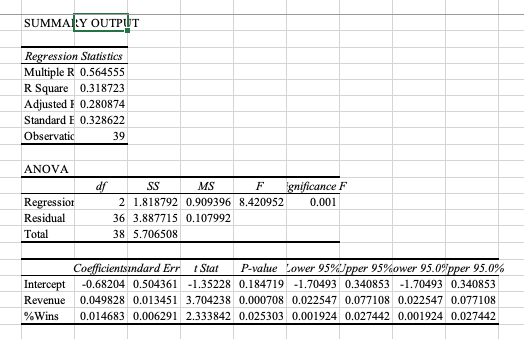
\includegraphics[scale=0.5]{Imagenes/50-24.png}
    \end{center}
    $$y= 0,049828x_1+0,014683x_2-0,68204$$
    \item Use la prueba F para determinar la significancia global de la relación. ¿Cuál es su conclusión empleando 0.05 como nivel de significancia?
    \begin{solution}
    La hipótesis nula se rechaza por el Valor-P, aunque es evidencia que la relación es significante.
    \end{solution}
    \item Utilice la prueba t para determinar la significancia de cada una de las variables indepen- dientes. ¿Cuál es su conclusión con un nivel de significancia de 0.05?
    \begin{solution}
    Dados los valores-P de las dos variables independientes y menores a 0.05, se concluye que son significantes.
    \end{solution}
\end{itemize}
\subsection{Ejercicio 51}
\begin{itemize}
   \item  Calcule las entradas que faltan en esta pantalla.
    \begin{center}
        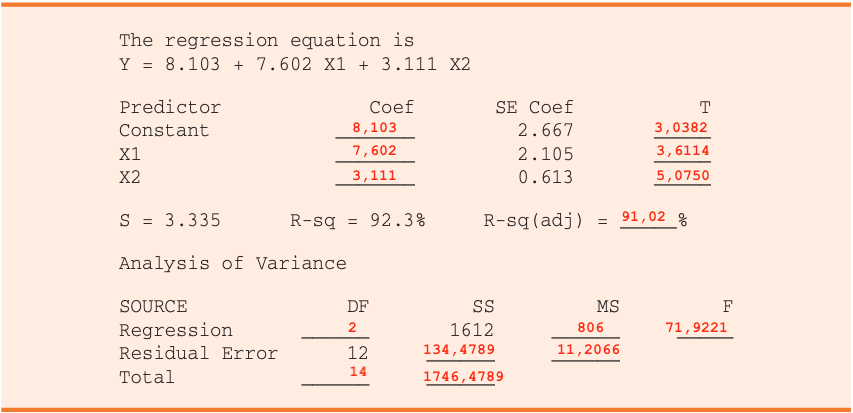
\includegraphics[scale=0.5]{Imagenes/50-51.png}
    \end{center}
   \item Use la prueba F y $\alpha= 0.05$ para identificar si existe una relación significativa.
   \begin{solution}
   Se rechaza la $H_0$ y se determina que es significante.
   \end{solution}
   
   \item  Utilice la prueba t y $\alpha =0.05$ para demostrar $H_0: \beta_11=0$ y $H_0:\beta_2=0$
   \begin{solution}
   Las variables $X_1$ y $X_2$ son significativas debibo a su valor-P mayor a 0.05. 
   \end{solution}
  
   \item Calcule $R^2_a$.
   
   $$
R_{a}^{2}=1-\left(1-R^{2}\right) \frac{n-1}{n-p-1}=1-(1-0.923) \frac{15-1}{15-2-1} \approx 0.9102=91.02 \%
$$
   
\end{itemize}


\subsection{Ejercicio 52},

\begin{itemize}
    \item Calcule las entradas que faltan en esta pantalla.
    \begin{center}
        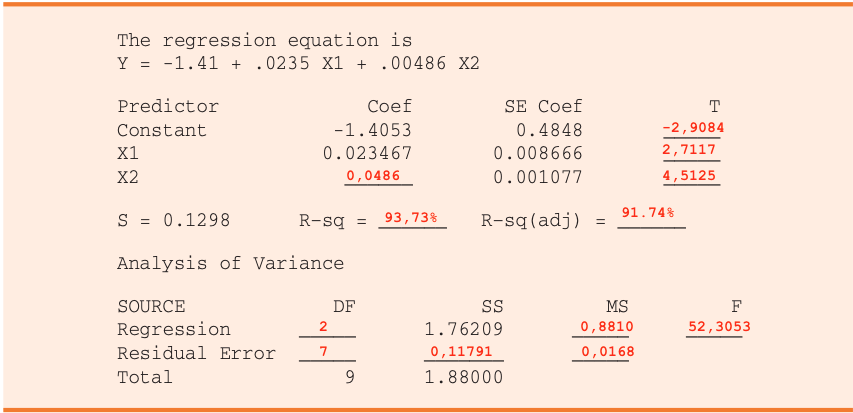
\includegraphics[scale=0.5]{Imagenes/50-52.png}
    \end{center}
    \item  Use la prueba F y 0.05 como nivel de significancia para saber si existe una relación significativa.
    \begin{solution}
    Basándose en la prueba F, hay suficiente evidencia para afirmar que la relación es significante.
    \end{solution}
    \item  Utilice la prueba t y $\alpha= 0.05$ para probar $H_0: \beta_1=0$ y $H_a: \beta_2= 0$.
    \begin{solution}
    Hay evidencia para afirmar que $X_2$ es significante, mientras que $X_1$ no lo es.
    \end{solution}
   \item  ¿La ecuación de regresión estimada proporciona un buen ajuste a los datos? Explique.
   \begin{solution}
   Basándose en $R^2$ y $R^2_a$ se puede afirmar que la ecuación de la regresión estimada tiene un buen ajuste.
   \end{solution}
\end{itemize}


\section{Sección 16}

\subsection{Ejercicio 11}
En un análisis de regresión con 30 observaciones se obtuvo la siguiente ecuación de regresión estimada.
$$
\hat{y}=17.6+3.8 x_{1}-2.3 x_{2}+7.6 x_{3}+2.7 x_{4}
$$
Para esta ecuación de regresión estimada, $\mathrm{STC}=1805 \mathrm{y} \mathrm{SCR}=1760 .$
\begin{itemize}
   
\item  $\quad$ Con $\alpha=0.05,$ pruebe la significancia de la relación entre las variables. Suponga que las variables $x_{1}$ y $x_{4}$ se retiran del modelo y se obtiene la siguiente ecuación de regresión estimada.
$$
\hat{y}=11.1-3.6 x_{2}+8.1 x_{3}
$$
Para este modelo, $\mathrm{STC}=1805$ y $ \mathrm{SCR}=1705 .$

\begin{solution}
\begin{align}
\begin{aligned}
M S E &=\frac{S S E}{n-p-1} =\frac{S S T-S S R}{n-p-1} =\frac{1805-1760}{30-4-1} =1.8 
& \\
M S R &=\frac{S S R}{p} 
=\frac{1760}{4} 
=440 \\
& \\
F&=\frac{M S R}{M S E} 
=\frac{440}{1.8}
=244.4444
\end{aligned}
\end{align}
Se rechaza la $H_0$ y se concluye que la relación es significativa.
\end{solution}
\item  $\quad$ Calcule $\operatorname{SCE}\left(x_{1}, x_{2}, x_{3}, x_{4}\right)$
\begin{solution}
$$SSE= SST-SSR = 45$$
\end{solution}
\item  $\quad$ Calcule $\operatorname{SCE}\left(x_{2}, x_{3}\right)$

\begin{solution}
$$SSE= SST-SSR = 100$$
\end{solution}
\item  Utilice la prueba $F$ y 0.05 como nivel de significancia para determinar si $x_{1}$ y $x_{2}$ contribuyen significativamente al modelo.
\begin{solution}
\begin{align}
\begin{aligned}
F &=\frac{\frac{\operatorname{SSE}\left(x_{2}, x_{3}\right)-\operatorname{SSE}\left(x_{1}, x_{2}, x_{3}, x_{4}\right)}{número de términos extra}}{\frac{\operatorname{SSE}\left(x_{1}, x_{2}, x_{3}, x_{4}\right)}{n-p-1}} \\
&=\frac{\frac{100-45}{2}}{\frac{45}{30-4-1}} \\
& \approx 15,2778
\end{aligned}
\end{align}
Se concluye que las variables son significativas.
\end{solution}
\end{itemize}
\subsection{Ejercicio 12}

\begin{itemize}
    \item Desarrolle una ecuación de regresión estimada para pronosticar la Scoring Avg. de todos los eventos dado el número promedio de putts en los golpes dados en Green in Reg.
    \begin{center}
        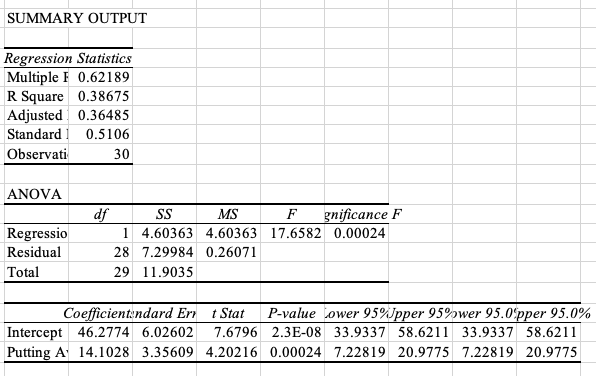
\includegraphics[scale=0.5]{Imagenes/60-10.png}
    \end{center}
    $$y=14,1028x+46,2774$$
    \item Desarrolle una ecuación de regresión estimada para pronosticar la Scoring Avg. de todos los eventos dado el tiempo promedio en que una jugadora es capaz de golpear el Green in Reg, y el promedio de veces en que consigue “subir y bajar” una vez que se encuentra en la trampa de arena.
    \begin{center}
        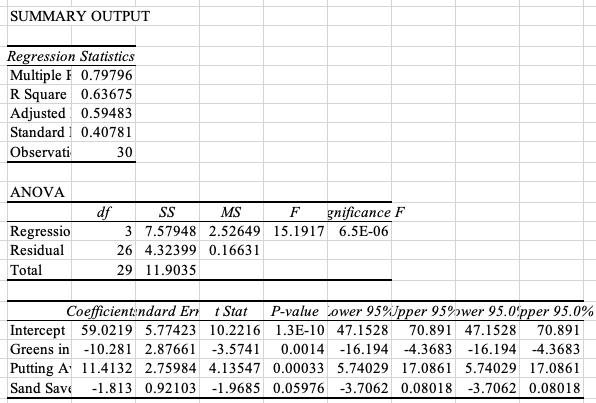
\includegraphics[scale=0.5]{Imagenes/60-10-2.png}
    \end{center}
    $$y=-10,281x_1+11,4132x_2-1,813x_3+59,0219$$
    \item Con un el nivel de significancia de 0.05, pruebe si las dos variables independientes agregadas en el inciso el porcentaje de veces en que una jugadora consigue llegar al green en regulación y el promedio de veces en que es capaz de “subir y bajar” una vez que se encuentra en la trampa de arena al lado del green, contribuyen significativamente el desarrollo de la ecuación de regresión en el inciso a). Explique.
    \begin{solution}
    

    \begin{align}
\begin{aligned}
F &=\frac{\frac{\operatorname{SSE}\left(x_{2}\right)-\operatorname{SSE}\left(x_{1}, x_{2}, x_{3}\right)}{\text { número de términos extra }}}{\frac{\operatorname{SSE}\left(x_{1}, x_{2}, x_{3}\right)}{n-p-1}} \\
&=\frac{\frac{7.2998-4.3240}{2}}{\frac{4.3240}{30-3-1}}\\
&= 8,9468
\end{aligned}
\end{align}

Por lo que se concluye, que es una regresión significativa.
 \end{solution}
\end{itemize}
\subsection{Ejercicio 14}
\begin{itemize}
    \item  Desarrolle una ecuación de regresión estimada para predecir el riesgo de fumar dada la edad y el nivel de presión sanguínea.
    \begin{center}
        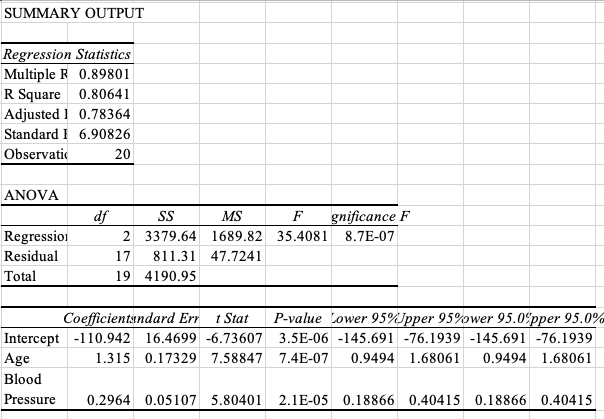
\includegraphics[scale=0.5]{Imagenes/60-14.png}
    \end{center}
    $$y=1,315x_1+0,2964x_2-110,942$$
    \item  Considere la adición de dos variables independientes al modelo desarrollado en el inciso a): una para la interacción entre la edad y el nivel de presión arterial y otra que indique si la persona es fumadora. Desarrolle una ecuación de regresión estimada utilizando estas cuatro variables independientes.
    \begin{center}
        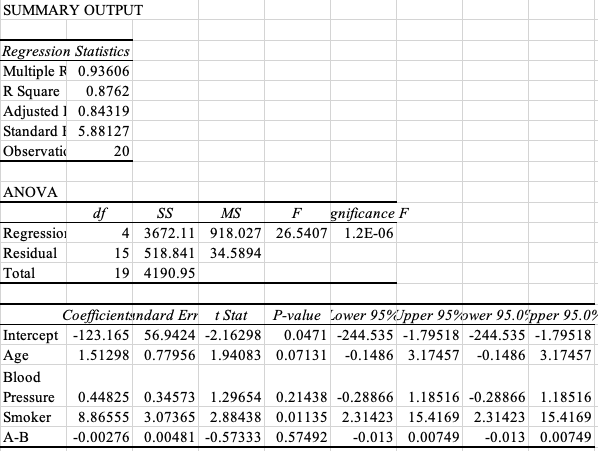
\includegraphics[scale=0.5]{Imagenes/60-27.png}
    \end{center}
    $$y=-0,00276x_4+8,86555x_3+0,44825x_2+1,51298x_1-123,165$$
    \item   Con un nivel de 0.05 de significancia, lleve a cabo una prueba para determinar si la adición del término interacción y la variable fumador contribuyen significativamente a la ecuación de regresión estimada desarrollada en el inciso a).
    \begin{solution}
    \begin{align}
\begin{aligned}
F &=\frac{\frac{\operatorname{SSE}\left(x_{1}, x_{2}\right)-\operatorname{SSE}\left(x_{1}, x_{2}, x_{3}, x_{4}\right)}{\operatorname{númbero} \text {de términos extra }}}{\frac{\operatorname{SSE}\left(x_{1}, x_{2}, x_{3}, x_{4}\right)}{n-p-1}} \\
&=\frac{\frac{811.3097-518.8406}{2}}{\frac{518.8406}{20-4-1}}\\
&= 4,2277
\end{aligned}
\end{align}

Por lo tanto, es significativo.
    \end{solution}
    
\end{itemize}

\subsection{Ejercicio 17}
The Ladies Professional Golfers Association (LPGA) lleva estadísticas sobre el desempeño y las ganancias de los miembros del LPGA Tour. Las estadísticas de fin de año sobre el papel de las 30 jugadoras que obtuvieron las mejores ganancias totales en la LPGA Tour de 2005 apArecen en el archivo titulado LPGATour2 (sitio web de LPGATour, 2006). Earnings (ganancias) constituyen el resultado total en miles de dólares en todos los eventos de la gira; Scoring Avg. es la puntuación promedio para todos los eventos; Drive Average es la distancia promedio en yardas alcanzada en el drive por la jugadora; Greens in Reg. es el porcentaje de veces que la golfista llega al green en regulación; Putting Avg. es el promedio de putts en el green en regulación, y Sand Saves es el porcentaje de veces que una jugadora es capaz de logra “subir y bajar” (up and down) cuando se encuentra en la trampa de arena al lado del green. Éste se considera un golpe en la regulación si alguna parte de la bola toca la superficie del putting y la diferencia entre el valor del par de hoyos y el número de golpes que lleva a golpear el green es por lo menos de 2. DriveGreens denota una nueva variable independiente que representa la interacción entre la distancia media alcanzada en el drive por la jugadora y el porcentaje de veces que es capaz de alcanzar el green en regulación. Utilice los métodos de esta sección a efecto de desarrollar la mejor ecuación de regresión múltiple estimada para calcular el Scoring Avg. de una jugadora en todos los eventos.

\begin{solution}
Matriz de correlación:
\begin{center}
    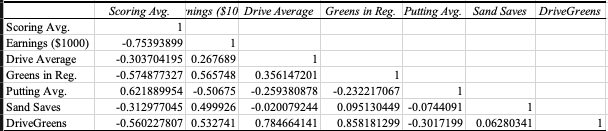
\includegraphics[scale=0.5]{Imagenes/70-1.png}
\end{center}
Por otra parte, la regresión lineal: 
\begin{center}
    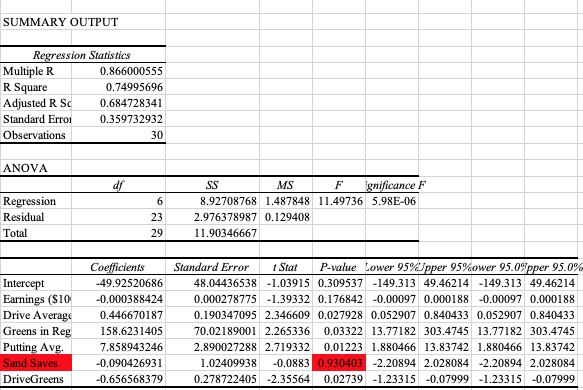
\includegraphics[scale=0.5]{Imagenes/70-3.png}
\end{center}

Se determinó que el valor-P de la variable Sand Saves es demasiado elevado, por lo que se decidió eliminarlo. 

\begin{center}
    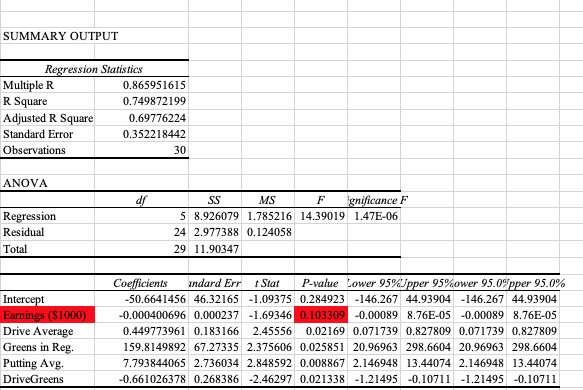
\includegraphics[scale=0.5]{Imagenes/70-4.png}
\end{center}

Por otra parte, también se determinó que la variable Earnings, tiene un Valor-P superior a 0.05, por lo que se decidió eliminarlo. 

\begin{center}
    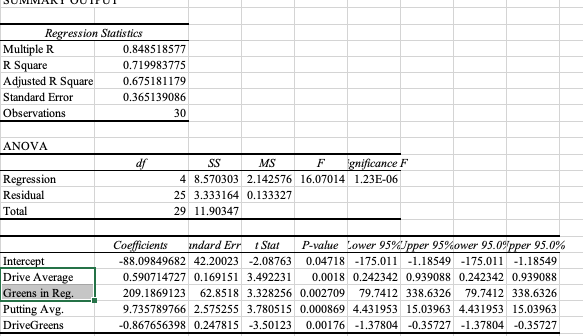
\includegraphics[scale=0.5]{Imagenes/70-5.png}
\end{center}

Finalmente, se llegó a un modelo de 4 variables, considerando:
\begin{itemize}
    \item Drive Average = $x_1$
    \item Greens in Reg = $x_2$
    \item Putting Avf = $x_3$
    \item DriveGreen = $x_4$
\end{itemize}
$$\implies y=0,5907x_1+209,1869_2+9,7378x_3-0,8676x_4-88,0984$$




\end{solution}







\end{document}